% ═══════════════════════════════════════════════════════════
% Three-Layer Progressive Optimization for Consumer-GPU GRPO
% v2 (journal-standard expansion). Compile: pdflatex → bibtex → pdflatex ×2
% Every reported number is traceable to results/efficiency/** or docs/19–21.
% ═══════════════════════════════════════════════════════════
\documentclass[11pt]{article}
\usepackage[margin=1in]{geometry}
\usepackage[T1]{fontenc}
\usepackage{mathptmx}
\usepackage[round,authoryear,sort&compress]{natbib}
\usepackage{booktabs}
\usepackage{array}
\usepackage{multirow}
\usepackage{graphicx}
\usepackage{amsmath,amssymb}
\usepackage{amsthm}
\usepackage{xcolor}
\usepackage{subcaption}
\usepackage{enumitem}
\usepackage[hidelinks]{hyperref}

\newtheorem{theorem}{Theorem}
\newtheorem{corollary}[theorem]{Corollary}
\newtheorem{proposition}[theorem]{Proposition}
\newtheorem{lemma}[theorem]{Lemma}
\theoremstyle{definition}
\newtheorem{assumption}{Assumption}
\graphicspath{{figures/}}

\newcommand{\fzs}{\text{fzs}}

\title{\textbf{Three-Layer Progressive Optimization:\\
Systematic Limit Approximation for Consumer-GPU\\
GRPO Post-Training}}
\author{Hongyu Chen}
\date{}

\begin{document}
\maketitle
\vspace{-2em}
\begin{center}\small
\textbf{DOI:} \href{https://doi.org/10.5281/zenodo.21947489}{10.5281/zenodo.21947489} \quad
\textbf{Code \& data:} \href{https://github.com/ChenHongYu2026/llm-training-on-consumer-amd}{github.com/ChenHongYu2026/llm-training-on-consumer-amd}
\end{center}
\vspace{1em}

\begin{abstract}
Can a single consumer GPU (AMD RX 7900 XTX, 24\,GB) perform effective reinforcement
learning from verifiable rewards (RLVR) for large language models? We present a
systematic three-layer optimization framework that progressively approaches the
theoretical limit at each layer before descending to the next.
(1) A \emph{throughput layer} (Decoupled-Generation Batch-Balancing, DGBB): a
three-parameter step-time law and a memory model jointly identify the true
two-dimensional feasible region of GRPO batch scheduling; under the hardware wall
the measured optimum (795.5\,tok/s) reaches 97.6\% of the within-wall theoretical
argmax, confirmed by pre-registered blind predictions and a probe experiment that
falsifies the naive extrapolation.
(2) A \emph{signal-rate layer} (Zero-Signal Budget Reallocation, ZSBR): a capacity
theory with an honest bound staircase and a closed-form Beta-posterior-expectation
scorer reach 94\% of the attainable $G{=}2$ signal-rate capacity at zero throughput
cost, yielding $+7.8$\,pp held-out accuracy over uniform sampling (Cohen's
$d{=}7.52$, three seeds, paired).
(3) A \emph{dynamics layer} (Signal-Flux Optimal Control, SFOC): a three-pool ODE
model of prompt-pool dynamics yields the $\tau_{net}$ regime criterion,
cross-validated by four independent estimates of the relay rate $\mu_0$, and a
\textbf{Scheduler-Constraint Capping Theorem} (proved) showing that
depletion-dominated dynamics is structurally unreachable under cooldown-based
scheduling. Across 20+ controlled runs on GSM8K with Qwen2.5-3B-Instruct, we
advance from a 23.2\% base to 45.6\% ($2\times$ pure-RL gain, 8.5\,h on one card),
show that 500 well-chosen prompts match the full 7473-pool ($15\times$ data
efficiency), and establish that greedy selection is strictly optimal in all
empirically observed regimes. All 13 pre-registered falsifiable predictions of the
first round converge to one self-consistent picture; two pre-registered follow-up
rounds (cooldown-removal falsification test; cross-architecture transfer to
Gemma~4~E2B, where DGBB re-fits at $R^2{=}0.9983$) confirm the capping theorem and
locate the model-specific parameters that must be recalibrated. Negative results
are reported in full and drive every theoretical refinement. We release the paper,
the complete training prompt pool, all evaluation artifacts, and the training and
evaluation code.
\end{abstract}

\section{Introduction}\label{sec:intro}
Reinforcement learning from verifiable rewards (RLVR) has become a primary driver
of reasoning improvements in large language models: group-relative methods such as
GRPO~\citep{shao2024grpo} replace learned value functions with within-group
relative advantages computed from rule-checkable rewards, and have been adopted at
scale in recent reasoning systems~\citep{yu2025dapo}. However, the dominant
practice assumes multi-GPU training clusters with hundreds of gigabytes of
aggregate memory, implicitly treating RLVR as a luxury affordable only at
data-center scale.

We ask a deliberately inconvenient question: \textbf{can RLVR be made effective on
a single consumer-grade GPU?} Consumer hardware differs from clusters in three
structural ways: no tensor parallelism (the whole model must fit in one card's
memory), a thinner software ecosystem (ROCm vs.\ CUDA), and sequential execution in
which throughput and signal quality compete for the same GPU-seconds. Any positive
answer must therefore be \emph{earned} layer by layer rather than assumed.

Our answer is affirmative, and it comes with a methodology: \textbf{three-layer
progressive optimization}. At each layer we (i) formalize the layer's theoretical
limit, (ii) measure how close the current system is to it, (iii) close the gap as
far as the layer's structure allows, and only then (iv) descend to the next layer,
where the remaining bottleneck lives. This discipline has a concrete payoff: when
each layer is saturated before descending, every claim about ``what works'' is
backed by an exhaustion argument about ``why nothing else at that layer can work''.
Figure~\ref{fig:milestone} summarizes the resulting ladder: held-out accuracy on
GSM8K doubles from a 23.2\% base to 45.6\% under pure RL on one consumer card.

\begin{figure}[t]
\centering
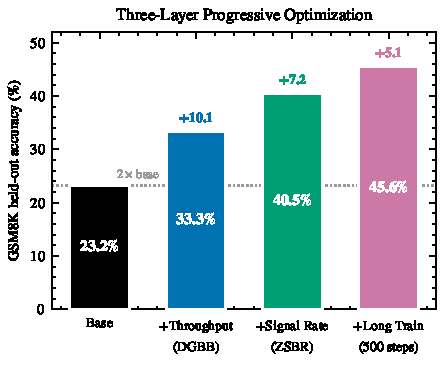
\includegraphics[width=0.72\linewidth]{fig1_milestone.pdf}
\caption{Three-layer progressive optimization on GSM8K + Qwen2.5-3B-Instruct.
Each layer's advance is justified by the exhaustion of the previous layer's
capacity: throughput saturates at 97.6\% of the hardware-wall limit before the
signal-rate layer begins; the signal rate reaches 94\% of its $G{=}2$ capacity
before the dynamics layer begins. Held-out accuracy doubles from the 23.2\% base
to 45.6\%.}
\label{fig:milestone}
\end{figure}

\paragraph{Contributions.}
\begin{enumerate}[leftmargin=1.5em]
\item \textbf{Throughput layer (\S\ref{sec:l1}).} A three-parameter step-time law
$T_{step}=a_1+a_2 B_g+a_3(B_g/B_b)$ and a piecewise-linear memory model identify
the two independent batch dimensions of GRPO (generation batch $B_g$, backward
micro-batch $B_b$). Pre-registered blind predictions, a probe experiment that
falsifies the naive large-$B_b$ extrapolation, and a dual-wall memory analysis
together establish that the measured optimum (795.5\,tok/s) is 97.6\% of the
within-wall theoretical argmax---the batch-scheduling dimension is exhausted.
The functional form transfers to a second model family at $R^2{=}0.9983$.
\item \textbf{Signal-rate layer (\S\ref{sec:l2}).} A capacity theory with an
honest bound staircase (including a proof that multi-selection cannot raise the
group-level signal rate) and a Beta-posterior-expectation scorer whose necessity
is demonstrated by a controlled ablation (point estimator fails, posterior
estimator succeeds). ZSBR reaches 94\% of the attainable $G{=}2$ capacity at zero
throughput cost; three-seed paired comparison gives $+7.8$\,pp ($d{=}7.52$).
\item \textbf{Dynamics layer (\S\ref{sec:l3}).} A three-pool ODE model of how
training modifies the prompt-pool pass-rate distribution; the $\tau_{net}$ regime
criterion with $\mu_0$ cross-validated on four independent paths; and a
\emph{proved} Scheduler-Constraint Capping Theorem showing that depletion-dominated
dynamics is structurally unreachable under cooldown-based greedy scheduling.
\item \textbf{Practice (\S\ref{sec:find}).} 23.2\%$\to$45.6\% in 8.5\,h of pure RL
on one consumer card; $15\times$ data efficiency (500 prompts $\approx$ full
7473-pool); and the first explicit ``when NOT to use curriculum'' criterion.
\item \textbf{Methodology (\S\ref{sec:method}).} A pre-registration-and-audit
protocol under which all 13 first-round predictions were judged against
timestamped thresholds, every negative result triggered a documented theoretical
refinement, and the final audit round closed with zero defects.
\end{enumerate}

\paragraph{Paper roadmap.} Section~\ref{sec:bg} fixes notation and positions the
work relative to prompt-selection and efficient-RL literature. Sections~\ref{sec:l1}--\ref{sec:l3}
develop the three layers in dependency order. Section~\ref{sec:find} collects the
practical implications; Section~\ref{sec:method} describes the methodology;
Sections~\ref{sec:threats}--\ref{sec:limits} cover threats to validity and
limitations. Appendices contain the complete prediction scorecard, phase-diagram
data, and the run inventory.

\section{Background and Related Work}\label{sec:bg}

\subsection{GRPO and the signal event}\label{sec:bg-grpo}
GRPO generates $G$ completions per prompt, computes within-group relative
advantages, and updates the policy without a value network. For a prompt $q$ with
per-completion reward distribution $\pi_q$ over a finite support $R$, the
probability that a group yields a \emph{non-zero} advantage---the \emph{signal
event}---is
\begin{equation}\label{eq:psig-exact}
P_{sig}(q) = 1 - \sum_{r \in R} \pi_q(r)^{G}.
\end{equation}
Under the binary approximation with pass rate $p_q$ this reduces, for $G{=}2$, to
\begin{equation}\label{eq:psig-binary}
P_{sig}(q) \approx 1 - p_q^{2} - (1-p_q)^{2} = 2p_q(1-p_q),
\end{equation}
maximized at $p_q{=}0.5$ (\emph{boundary} prompts) and vanishing for prompts that
are consistently solved or consistently failed. Two facts make this quantity the
organizing concept of the paper. First, at $G{=}2$ on our base model we measure
$\text{frac\_reward\_zero\_std}{=}0.75$ across configurations---\emph{75\% of the
generated compute produces zero-gradient groups} (\S\ref{sec:l2}). Second,
$P_{sig}$ depends on $G$ and $\pi_q$ but not on the generation batch size, a
prediction we verify explicitly (Appendix scorecard, P6).

\subsection{Related work}\label{sec:bg-related}
\paragraph{Prompt selection and zero-variance filtering.}
GRESO~\citep{zheng2025greso} filters zero-variance prompts pre-rollout using
historical reward dynamics across epochs, and observes that the effective-prompt
ratio decays during training without modeling that decay. Our work independently
reached the same direction from a hardware-measurement starting point
(\S\ref{sec:l2}); we contribute a decision-theoretic scorer with a controlled
necessity ablation, a capacity theory with explicit attainable bounds, and a
dynamics theory for the decay GRESO observes.
DAPO~\citep{yu2025dapo} instead filters zero-advantage groups \emph{post}-rollout
and oversamples to refill; \S\ref{sec:l2-dapo} gives a cost comparison (pre- vs.\
post-rollout filtering). PCL~\citep{gao2025pcl} trains a value model to select
medium-difficulty prompts---myopic with respect to pool depletion. RL-ZVP
\citep{le2025rlzvp} keeps zero-variance prompts and shapes their advantages via
entropy; this modifies gradients rather than budget allocation, and our negative
results delineate its regime of applicability (investing in zero-signal prompts is
net-harmful when supply dominates; \S\ref{sec:l3-invest}). SRPO~\citep{li2026srpo}
routes samples to self-distillation, an orthogonal direction.

\paragraph{Curriculum and data selection for RL.} The Implicit Curriculum
\citep{huang2026implicit} gives a descriptive theory of relay effects under uniform
training---easy problems' persistent gradients make slightly harder problems
learnable---and is the theoretical foundation for our relay (supply) term $\mu_0$;
it contains no control variable and no depletion analysis. Our contribution is the
\emph{normative} counterpart: budget allocation as optimal control on pool
dynamics, a quantitative regime criterion, and an impossibility result
(\S\ref{sec:l3}).

\paragraph{Efficient RL systems.} Systems work on RL training efficiency
(e.g., generation--training co-scheduling and rollout acceleration) targets
clusters; the consumer-GPU constraint set (single card, no tensor parallelism,
memory wall at 24\,GB) makes the three-layer decomposition---throughput $\times$
signal rate $\times$ dynamics---the natural optimization structure, since all three
resources are the \emph{same} GPU-seconds.

\paragraph{Positioning.} To our knowledge this is the first work to (a) model RLVR
prompt-budget allocation as non-myopic optimal control on pool dynamics, (b) derive
a quantitative regime criterion ($\tau_{net}$) with multi-path parameter
validation, and (c) prove a structural-impossibility theorem for depletion under
realistic scheduling. A pre-writing literature search and a post-experiment
novelty re-audit are documented in the methods appendix (\S\ref{sec:method}); the
re-audit corrected one overclaim (GRESO priority on pre-rollout filtering), which
we record as part of the protocol's output.

\subsection{Consumer-GPU constraints}\label{sec:bg-hw}
The RX 7900 XTX (RDNA3, gfx1100) provides 24\,GB VRAM, 960\,GB/s nominal memory
bandwidth (742\,GB/s measured on pure copies, 77\%), and 101.53\,TFLOPS measured
BF16 GEMM peak. Against training clusters: (i) no tensor parallelism---all weights
must reside on one card; (ii) ROCm ecosystem gaps versus CUDA (kernel coverage,
allocator behavior); (iii) single-card sequential execution, so throughput
improvements and signal-quality improvements spend the same budget. Batch-1
decoding is bandwidth-bound at only 38\% of achievable bandwidth
(\S\ref{sec:l1-roofline}), which is why generation-heavy GRPO is dominated by
decoding and why batch scheduling is the first lever.


\section{Layer 1: Throughput --- DGBB}\label{sec:l1}

\subsection{Two-dimensional decoupling}\label{sec:l1-decouple}
In generation-heavy GRPO the step time is decoding-dominated. Standard trainers
expose a single batch knob, but TRL's semantics (\texttt{generation\_batch\_size}
$=$ \texttt{per\_device\_batch} $\times$ \texttt{grad\_accum}) reveal two
\emph{independent} dimensions: the generation batch $B_g$ (arithmetic intensity of
the rollout phase) and the backward micro-batch $B_b$ (parallelism of the gradient
phase), constrained only by $B_b \mid B_g$. Decoupled-Generation Batch-Balancing
(DGBB) treats $(B_g, B_b)$ as two optimization variables. Crucially, this
decoupling changes no algorithmic semantics---update rule, sample distribution,
and optimization trajectory are identical to standard GRPO; the throughput gain is
free.

\paragraph{Step-time model.} Each optimization step is one generation phase plus
$B_g/B_b$ backward micro-batches plus constant overhead:
\begin{equation}\label{eq:tstep-struct}
T_{step}(B_g,B_b) = T_{gen}(B_g) + \frac{B_g}{B_b}\,T_{bwd}(B_b) + c .
\end{equation}
Roofline reasoning gives first-order phase structure $T_{gen}(B)=\alpha_g+\beta_g B$
(fixed weight reads plus per-sequence marginal cost) and
$T_{bwd}(b)=\delta+\gamma b$ (per-micro-batch overhead plus per-sequence marginal
cost). Substituting into \eqref{eq:tstep-struct} yields the three-parameter
identifiable form
\begin{equation}\label{eq:tstep}
T_{step} = a_1 + a_2 B_g + a_3\frac{B_g}{B_b}, \qquad
a_1=\alpha_g+c,\; a_2=\beta_g+\gamma,\; a_3=\delta,
\end{equation}
where $a_3$ quantifies why $B_b{=}1$ is inefficient. Throughput is
$\mathrm{TPS}=k_{tok}B_g/T_{step}$ with $k_{tok}$ the tokens-per-sequence count
(measured 355.7, $\approx$108 prompt + 247 completion tokens).

\paragraph{Independent roofline validation of the generation phase.}
\label{sec:l1-roofline}
A pure-decoding microbenchmark (SDPA + static cache, batch $\in\{1,\dots,64\}$)
fits $t_{dec}(B)=21.63+0.413B$ ms per decoding step. The intercept corresponds to
reading all 6.17\,GB of weights per step at an effective 285\,GB/s---only 38\% of
the 742\,GB/s pure-copy bandwidth; this is the roofline statement of the batch-1
GEMV inefficiency. The model's internal consistency check also holds:
$a_2\approx\beta_g+\gamma$ with $\beta_g\approx0.413\,\text{ms}\times 247$
decoding steps $\approx0.102$\,s/seq recovers $\gamma\approx0.256$\,s/seq for the
backward phase, whose implied backward MFU ($\approx$25\%, from
$6N\bar L\approx6.6$\,TFLOP per sequence) is plausible under LoRA plus gradient
checkpointing.

\subsection{Memory model and the dual wall}\label{sec:l1-mem}
Peak VRAM is the maximum of the two phases' peaks:
\begin{equation}\label{eq:mem}
M(B_g,B_b) = m_0 + m_g B_g + m_b\max(0, B_b - B_{th}),
\end{equation}
fitted at $m_0{=}6.57$\,GB (weights 6.17\,GB BF16 plus LoRA, optimizer, and
resident state), $m_g{=}0.03625$\,GB per sequence, $m_b{=}0.46$\,GB per sequence,
and $B_{th}{=}4$, with per-point residuals within 0.05\,GB. Because gradient checkpointing compresses backward
activations, for $B_b\le4$ the generation phase dominates the peak and
\emph{$B_b$ 1$\to$4 costs zero memory} (measured 8.87\,GB identical across three
settings)---the memory-side mechanism behind ``the backward batch is a free
lever''.

A pre-registered blind prediction then exposed the model's boundary: the naive
feasibility criterion predicted gen384 runnable at 20.49\,GB, but the run OOMed.
Post-hoc analysis of the OOM logs (treated as data) gives the corrected criterion
$M_{steady}+M_{spike}+M_{sys}\le24$\,GB with a one-shot allocation spike
$M_{spike}\approx3.8$\,GB at $B_g{=}384$ (logits/attention intermediates) and
$M_{sys}\approx1.5$--$2$\,GB outside the allocator's visibility. The corrected
wall lands in $(256,384]$ tokens---matching measurements---and a controlled re-run
showed the default allocator's fragmentation wall (3.9\,GB lost) is distinct from
the capacity wall and is removed by \texttt{expandable\_segments}. The companion
prediction (gen512 $\to$ 25.13\,GB $\to$ OOM) hit exactly.

\subsection{Fit quality and falsification of the naive extrapolation}\label{sec:l1-fit}
Fitting \eqref{eq:tstep} on the seven feasible sweep points gives
$a_1{=}10.829$\,s, $a_2{=}0.3579$\,s/seq, $a_3{=}0.1702$\,s/micro-batch, with all
residuals within $\pm$3.3\%. The pre-registered model's argmax under the empirical
wall was pdb8\_gen256 at a predicted 843.9\,tok/s ($+6\%$ over the measured best);
a dedicated probe run measured $(B_b,B_g){=}(8,256)$ at 794.3\,tok/s---statistically
tied with pdb4's 795.5 (0.15\% difference, far below the 1--4\% run-to-run CV) and
at identical peak memory (15.81 vs.\ 15.82\,GB), \emph{falsifying the linear
$T_{bwd}$ extrapolation}: sub-linear degradation at $b{>}4$ exactly cancels the
halved micro-batch count, so the argmax landscape is flat beyond $B_b{=}4$.
Re-fitting with the probe point ($a_3$ revised down 24\%, max residual 6.02\%)
confirms pdb4\_gen256 as the true argmax. Table~\ref{tab:util} summarizes the
resulting utilization hierarchy.

\begin{table}[t]
\centering\small
\caption{Utilization hierarchy of the batch-scheduling dimension (Qwen2.5-3B,
$k_{tok}{=}355.7$, 6ND-MFU against the 101.53\,TFLOPS measured GEMM peak). The
measured optimum sits within measurement noise of the within-wall argmax.}
\label{tab:util}
\begin{tabular}{@{}llcc@{}}
\toprule
Level & Description & tok/s & 6ND-MFU \\
\midrule
0 & Measured optimum (pdb4, gen256) & 795.5 & 14.5\% \\
1 & Within-wall theoretical argmax & 815.3 & 14.9\% \\
2 & Asymptotic, no memory wall ($B_b{=}4$, $B_g{\to}\infty$) & 864.8 & 15.8\% \\
3 & Zero micro-batch overhead ($B_b{\to}\infty$; probe-refuted in practice) & 939.0 & 17.2\% \\
4 & Kernel-level changes (faster backward, quantized generation) & $>$939 & --- \\
\bottomrule
\end{tabular}
\end{table}

\paragraph{Why the ceiling is structural.} Decomposing $a_2=\beta_g+\gamma$: 29\%
of per-sequence time is generation (memory-bound; MFU is not the right metric---by
bandwidth utilization, 38\% of achievable) and 71\% is backward (compute-bound at
$\approx$25\% MFU under gradient-checkpointing recomputation, LoRA branches, and
RDNA3 WMMA efficiency). The $\approx$18\% headroom above the measured optimum
therefore lives in kernels (level 4), not in batch scheduling: \emph{the
scheduling dimension is exhausted.} Mixed single-number MFU is misleading here;
per-phase accounting is the methodological point.

\subsection{Convergence theory: why throughput buys accuracy}\label{sec:l1-conv}
GRPO's per-step gradient over $B_g$ completions ($m{=}B_g/G$ unique prompts) has
$\mathrm{Var}[\hat g]\propto G/B_g$ by prompt-wise independence: gen8$\to$gen128
reduces variance $16\times$. Three registered checks confirm the mechanism:
(i) reward-curve variance ratio 9.2$\times$ (theory $16\times$, same order; the
floor comes from non-stationary learning drift and discrete reward support);
(ii) seed-to-seed dispersion of final accuracy \emph{halves} (1.14 vs.\ 2.25\,pp),
a pre-declared consequence of more deterministic trajectories; (iii) the
equal-sample adjudication run: gen128$\times$100 steps (34.6\%) vs.\
gen8$\times$1600 steps at equal 12\,800 samples (34.4\%)---large batches do
\emph{not} sacrifice per-sample learning efficiency, so throughput superiority
converts 1:1 into wall-clock convergence superiority ($\approx$1/5 wall clock).
Under equal \emph{step} budgets the paired multi-seed gain is $+3.9$\,pp
($d{=}2.66$), dominated by sample volume with variance reduction as the secondary
mechanism.

\subsection{Adopted configuration and cross-architecture replication}\label{sec:l1-adopt}
gen256 is VRAM-critical; the throughput--memory sweet spot gen128 (pdb4, ga32;
745.2\,tok/s at 11.26\,GB, $T_{step}\approx60$\,s) is adopted for all subsequent
training. On a second base model (Gemma~4~E2B, 1.6B-text multimodal) the same
decoupled form re-fits at $R^2{=}0.9983$:
$T_{step}=4.40+0.431\,B_g+0.174\,(B_g/B_b)$---the functional form is portable
with model-specific coefficients (prediction P-C1, \checkmark). The VRAM wall moves
to $\ge$512 tokens (16.4\,GB, no OOM) versus $(256,384]$ for Qwen, reflecting
architecture-specific memory efficiency. This upgrades DGBB from a single-model
case study to a portable throughput law.


\section{Layer 2: Signal Rate --- ZSBR}\label{sec:l2}
With throughput saturated, the next lever is not more compute but more
\emph{signal per compute}. At $G{=}2$ we measure
$\text{frac\_reward\_zero\_std}{=}0.75$ on the base model---75\% of generated
groups have identical within-group rewards, hence zero advantage and zero
gradient. Zero-Signal Budget Reallocation (ZSBR) predicts each prompt's signal
probability \emph{before} generation and reallocates the fixed group budget away
from predicted zero-signal prompts.

\subsection{Formalization and the uniform baseline}\label{sec:l2-form}
Let $Q$ be the prompt pool ($|Q|{=}7473$), $M{=}B_g/G{=}64$ the per-step group
budget, and rewards supported on $\{0,0.1,0.9,1.0\}$ (wrong / format-only /
approximate / correct). The exact signal probability is \eqref{eq:psig-exact}; the
binary approximation \eqref{eq:psig-binary} is a lower bound under 4-value
support (groups differing only in format, $\{0,0.1\}$, also produce signal).
Uniform sampling's system signal rate is $S_0=\mathbb{E}_{q\sim U}[P_{sig}(q)]
{=}0.25$ (calibrated from the measured zero-std fraction): only 16 of 64 group
slots carry gradient. The selection objective is
\begin{equation}\label{eq:zsbr-obj}
\max\; \bar S = \frac{1}{T}\sum_{t}\frac{1}{M}\sum_{q\in A_t} P_{sig}(q)
\quad \text{s.t.}\quad |A_t|=M,
\end{equation}
with $A_t$ the selected prompts at step $t$.

\subsection{Capacity theory: an honest bound staircase}\label{sec:l2-cap}
Claims about ``how much room is left'' require an explicit ledger.
Table~\ref{tab:staircase} records the staircase for $G{=}2$, distinguishing two
metrics that the literature often conflates: the \emph{group-level} signal rate
(the fraction of groups with non-zero advantage, directly measured as
$1-\fzs$) and the \emph{prompt-level coverage} (the probability that at least one
of a prompt's allocated groups signals).

\begin{table}[t]
\centering\small
\caption{Signal-rate capacity staircase ($G{=}2$). L4 requires per-prompt adaptive
$G$, which fixed-$G$ trainers cannot express without trainer surgery; the reachable
staircase under standard trainers ends at L1 for the group-level metric.}
\label{tab:staircase}
\begin{tabular}{@{}llccc@{}}
\toprule
Level & Mechanism & Group-level bound & Coverage bound & Reachable \\
\midrule
L0 & Uniform sampling & 0.25 & --- & baseline \\
L1 & Perfect selection (all $p{\approx}0.5$) & 0.50 & 0.50 & yes \\
L2 & Multi-selection $k{\le}2$ & 0.50 (no change) & 0.75 & yes \\
L3 & Multi-selection $k{\le}3$ & 0.50 (no change) & 0.875 & yes \\
L4 & Per-prompt adaptive $G$ & $\to1$ & $\to1$ & no \\
\bottomrule
\end{tabular}
\end{table}

Two declarations keep the ledger honest. \emph{First}, multi-selection cannot raise
the group-level rate: a prompt's second group has the same $P_{sig}$ as its first,
so extra slots increase the \emph{number of covered prompts} but not the fraction
of signaling groups---the group-level metric caps at L1$=$0.50 regardless of $k$
(this corrects an earlier overclaim in our own pre-registration, recorded as P5 in
the scorecard). \emph{Second}, L1 attainability depends on the empirical pass-rate
distribution: it requires $\ge M$ boundary prompts identifiable by the estimator.
Our deconvolved distribution (\S\ref{sec:l3-deconv}) contains ${\approx}3425$
boundary prompts $\gg M$, so the bound is active; ZSBR-V1 reaches $S{=}0.425$,
i.e., \textbf{94\% of the $\varepsilon$-adjusted L1 bound} (0.45 after reserving
$\varepsilon{=}0.2$ exploration; 85\% of the ideal 0.50).

\subsection{The estimator: why posterior expectation is necessary}\label{sec:l2-est}
Pass rates are estimated online with a Beta prior and time-decayed counts,
$\hat p_q = (\alpha_0+\gamma^{\Delta t}s_q)/(\alpha_0+\beta_0+\gamma^{\Delta
t}n_q)$, $\alpha_0{=}\beta_0{=}1$, $\gamma{=}0.98$ (half-life ${\approx}34$
cycles). Unseen prompts receive $\hat p{=}0.5$, making them maximally
attractive---optimistic cold start doubles as free exploration, no explicit UCB
needed.

\paragraph{Controlled ablation (point vs.\ posterior estimator).} Substituting the
point estimate into the non-linear map $p\mapsto2p(1-p)$ makes unseen prompts
($\hat p{=}0.5\Rightarrow\hat P_{sig}{=}0.5$) exactly tied with
\emph{confirmed} boundary prompts ($\hat p{=}0.5\Rightarrow\hat P_{sig}{=}0.5$);
with ${\approx}5000$ unseen vs.\ ${\approx}600$ mixed prompts, the greedy slots
flood with exploration and behavior degenerates to quasi-uniform (measured:
$\fzs{=}0.708$, coverage 0.614, pre-registered gate failed). The fix scores by
the Beta posterior expectation, available in closed form for $G{=}2$:
\begin{equation}\label{eq:posterior}
\mathbb{E}[P_{sig}\mid D]
= \mathbb{E}[2p(1-p)\mid D]
= \frac{2\alpha\beta}{(\alpha+\beta)(\alpha+\beta+1)},
\end{equation}
which orders mixed (0.400) $>$ unseen (0.333) $>$ consistent (0.300) and widens
with evidence (mixed seen twice: 0.4286). Under the identical configuration the
posterior estimator passes the gate ($\fzs{=}0.575$). To our knowledge this
paired failure/success is the first controlled demonstration that
\emph{uncertainty must enter the score} for small-sample RLVR scheduling.
A second calibration subtlety: the plug-in estimator $1-\sum_r\hat\pi_r^2$ carries
an $(n{-}1)/n$ small-sample bias---a factor of two at $n{=}2$---removed by the
standard unbiased correction.

\paragraph{Coverage and cooldown.} Pure greed has two failure modes: estimator
stagnation (out-of-distribution forgetting) and boundary-pool monopoly. An
$\varepsilon$-mix keeps $\varepsilon M$ slots uniform over the rest of the pool
(guaranteeing every prompt $\ge\varepsilon M/|Q|$ exploration probability per
step), and a cooldown $C{=}3$ cycles excludes recently used prompts from greedy
slots. The reward support is 4-valued, so a ``near-boundary'' wrong-but-answered
prompt still yields partial signal; the scheduler tracks this via the 4-value
posterior.

\subsection{V2 multi-selection: water-filling and its degeneration}\label{sec:l2-v2}
Since per-prompt $G$ is infeasible in fixed-$G$ trainers, V2 lets a prompt occupy
$k_q\le k_{max}{=}3$ group slots (each group sampled and normalized independently),
$\sum_q k_q = M$. A linear objective $\sum k_q P_{sig}(q)$ collapses all budget
onto one prompt; the correct objective is coverage
\begin{equation}\label{eq:waterfill}
v(q,k) = 1-(1-P_{sig}(q))^{k}, \qquad
\max \sum_q v(q,k_q)\;\; \text{s.t.}\;\; \sum k_q=M,\; 0\le k_q\le 3 .
\end{equation}
The marginal gain $\Delta v(q,k)=P_{sig}(q)(1-P_{sig}(q))^{k}$ is strictly
decreasing in $k$, so \eqref{eq:waterfill} is a separable concave maximization and
greedy water-filling is globally optimal.

\paragraph{Result and theoretical clarification.} V2 measured $\fzs{=}0.561$,
held-out 40.2\%, throughput $-1.4\%$---but with \emph{zero} duplicated slots.
This is not an implementation failure: with a boundary pool of 1549 prompts
$\gg 51$ greedy slots, the second-slot marginal $0.40\times0.60{=}0.24$ is always
below the next unseen prompt's $\ge0.333$, so the water-filling optimum
\emph{is} no duplication; V2 degenerates to V1 exactly as the mathematics
dictates. V2's applicability precondition---boundary pool smaller than the greedy
slot count (small datasets or late training)---was verified to hold later in the
pool-200 regime (\S\ref{sec:l3-regime}).

\subsection{Main results (three seeds, paired, same-round)}\label{sec:l2-results}
Table~\ref{tab:zsbr-main} reports the pre-registered comparison. All six
first-round predictions P1--P6 were timestamped before running
(Appendix~\ref{app:scorecard}); P1--P4 and P6 pass, P5 fails on a metric-confusion
in the prediction itself (recorded and corrected in \S\ref{sec:l2-cap}).

\begin{table}[t]
\centering\small
\caption{ZSBR-V1 vs.\ uniform sampling at equal step budget (100 steps) and equal
throughput. Held-out: GSM8K test[:500], batch 32, three seeds, paired by seed.
$\fzs$: fraction of zero-std groups, second half of training.}
\label{tab:zsbr-main}
\begin{tabular}{@{}lcccc@{}}
\toprule
Arm & Seed 42 & Seed 123 & Seed 7 & Mean $\pm$ std \\
\midrule
Uniform held-out & 31.0\% & 34.0\% & 33.2\% & 32.7\% $\pm$ 1.6 \\
ZSBR-V1 held-out & 39.6\% & 40.6\% & 41.4\% & 40.5\% $\pm$ 0.9 \\
\midrule
Paired difference & +8.6 & +6.6 & +8.2 & $+7.8$\,pp, $d{=}7.52$ \\
$\fzs$ (2nd half) & 0.575 & 0.573 & 0.575 & consistent to 0.2\,pp \\
$T_{step}$ change & \multicolumn{4}{c}{$-2.6\%$ (zero throughput cost)} \\
\bottomrule
\end{tabular}
\end{table}

Three structural observations: (i) the signal rate is consistent to 0.2\,pp across
seeds---it is an algorithm-structure quantity, in contrast with held-out
accuracy's seed stochasticity; (ii) ZSBR's seed dispersion (0.9\,pp) is
\emph{smaller} than uniform's (1.6\,pp)---high-signal training is more
reproducible, consistent with the variance theory of \S\ref{sec:l1-conv};
(iii) effective signal groups per second improve $1.75\times$ (0.450 vs.\
0.257) with coverage 0.224---low coverage plus high held-out simultaneously is
the algorithm's intent (budget concentration), not overfitting.

\subsection{Comparison with post-rollout filtering (DAPO)}\label{sec:l2-dapo}
DAPO-style dynamic sampling generates everything, discards zero-advantage groups,
and oversamples until $M$ effective groups are reached; its per-effective-group
generation cost is $1/S$ with variable step time and VRAM spikes. ZSBR's cost is
also $1/S_{ZSBR}$ per effective group but with \emph{constant} step time and VRAM
(orthogonal to the throughput layer's guarantees). At the achieved
$S_{ZSBR}{=}0.425$, matching uniform's effective-group output would cost DAPO
${\approx}1.66\times$ generation wall-clock; ZSBR pays zero wall-clock. The two
are composable (filter the zero-signal groups ZSBR misses); we leave this to
future work.

\subsection{Long training: the 45.6\% milestone}\label{sec:l2-long}
Extending ZSBR-V1 to 500 steps (8.5\,h, single card) without modification raises
held-out from 40.6\% (step-100 regime) to \textbf{45.6\%} (228/500; midpoint
checkpoint at step 250: 40.6\%, monotone, no overfitting signature; final KL
0.0070, reward 0.51). This is a $2\times$ pure-RL gain over the 23.2\% base and
remains the project's highest result. The signal rate does not decay over the
extension (fzs three segments 0.592/0.554/0.541, i.e., \emph{falling} zero-std
fraction = rising signal)---the observation that launches the dynamics layer.

\subsection{Cross-architecture transfer}\label{sec:l2-transfer}
On Gemma~4~E2B, $S_0{=}0.400$ (vs.\ 0.25 for Qwen): the base model already solves
more prompts, compressing the reallocation headroom (the $S_0$-compression
hypothesis, pre-registered). The 100-step transfer test measured uniform 29.27\%
vs.\ ZSBR 28.87\% ($-0.40$\,pp, $t{=}-0.53$; prediction P-C2 $\times$), but with a
$4\times$ variance reduction (ZSBR $\sigma{=}0.3$\,pp vs.\ uniform 1.2\,pp): when
signal is already abundant, reallocation \emph{stabilizes} rather than boosts mean
accuracy. The window may also be too short (Qwen's $+7.8$\,pp needed 500 steps).
Both caveats were declared pre-registration.


\section{Layer 3: Dynamics --- SFOC Phase Diagram}\label{sec:l3}
Layers 1--2 treat the prompt pool as static. But training modifies the model, and
the model modifies the pool: as pass rates rise, prompts migrate from hard (D)
through boundary (M) to learned (S). Selection is therefore simultaneously the
\emph{source} of reward and the \emph{driver} of the state it selects from---a
control problem, not a static knapsack. Signal-Flux Optimal Control (SFOC) makes
this explicit and asks: does the pool deplete, and can investment (spending budget
on hard prompts to convert them) ever pay off?

\subsection{Two-level state model and the observation problem}\label{sec:l3-deconv}
Let $p_q(t)$ be prompt $q$'s true per-completion pass rate and $\rho(p,t)$ the
population density. Coarse-grain into pools $D{=}[0,\delta)$,
$M{=}[\delta,1{-}\delta]$, $S{=}(1{-}\delta,1]$ with $\delta{=}0.15$. The system
signal rate is $S(t)=\int 2p(1-p)\rho(p,t)\,dp$ ($G{=}2$).

The pool labels used by any scheduler are \emph{observations}, not truth: one
selection produces $G{=}2$ binomial draws with confusion structure
\begin{equation}\label{eq:confusion}
P(\text{mixed}\mid p)=2p(1-p),\quad
P(\text{all-correct}\mid p)=p^2,\quad
P(\text{all-wrong}\mid p)=(1-p)^2 .
\end{equation}
A prompt at true $p{=}0.5$ is observed ``mixed'' only 50\% of the time. A
Beta-binomial EM deconvolution over the merged three-seed uniform logs (7454
prompts, ${\approx}6$ observations each) recovers the true pool composition
(Table~\ref{tab:deconv}): the true boundary pool is nearly \emph{twice} the
observed one (45.8\% vs.\ 24.2\%), because $n{=}2$ binomial noise mislabels half
of all boundary prompts as consistent. Cross-consistency check:
$S_{true}(\rho){=}0.2406$ predicts $\fzs{=}0.759$ vs.\ measured 0.7405. To our
knowledge this is the first quantification of how much small-$G$ observation noise
hides from curriculum-style schedulers.

\begin{table}[t]
\centering\small
\caption{Pool composition: observation labels ($n{=}2$) vs.\ Beta-binomial EM
deconvolution ($n{\approx}6$, three merged seeds).}
\label{tab:deconv}
\begin{tabular}{@{}lcc@{}}
\toprule
Pool & Observed & True (deconvolved) \\
\midrule
D (hard) & 50.5\% & 40.6\% \\
M (boundary) & 24.2\% & \textbf{45.8\%} \\
S (learned) & 25.3\% & 13.6\% \\
\bottomrule
\end{tabular}
\end{table}

\subsection{Three-pool ODE model and the decay law}\label{sec:l3-ode}
With cycle as the time unit and pool fractions $D{+}M{+}S{=}1$, control variables
$(a_M,a_D)$ (fractions of the per-cycle group budget $M_b{=}64$):
\begin{equation}\label{eq:ode}
\frac{dM}{dt} = \underbrace{\lambda_{DM}(a_D)\,D}_{\text{relay supply}}
- \underbrace{\lambda_{MS}(a_M)\,M}_{\text{harvest depletion}},\qquad
\begin{cases}
\lambda_{MS} = \mu_h\,\dfrac{a_M M_b}{|M|},\\[1.2ex]
\lambda_{DM} = \mu_0 + \mu_i\,\dfrac{a_D M_b}{|D|},
\end{cases}
\end{equation}
with constraint $a_M+a_D+\varepsilon=1$. Harvest moves boundary prompts to
learned at a rate proportional to per-prompt budget; supply has a natural
\emph{relay} term $\mu_0$ (the Implicit Curriculum effect: generalization on other
prompts converts hard prompts to boundary) and an investment term $\mu_i$.
Signal rate approximates $S(t)\approx s_M M(t)+s_\varepsilon$ ($s_M\approx0.45$).

\begin{proposition}[Decay law]\label{prop:decay}
Under myopic greedy selection ($a_D\equiv0$, the common form of
ZSBR/GRESO/PCL), the boundary pool obeys
\begin{equation}\label{eq:decay}
M(t) = M_0 e^{-t/\tau} + \frac{\mu_0 \bar D}{\lambda_{MS}}\left(1-e^{-t/\tau}\right),
\qquad \tau = \frac{|M|}{\mu_h M_b a_M}.
\end{equation}
If $\mu_0 \bar D \ll \lambda_{MS} M_0$ the pool depletes exponentially (fzs
rebound); if relay supply balances harvest, $M(t)$ plateaus at
$M_\infty=\mu_0\bar D/\lambda_{MS}$. \emph{Both outcomes are predictions of the
same model}; the regime is decided by measurement.
\end{proposition}
\begin{proof}
Linear ODE in $M$ with constant coefficients under fixed $(\bar D, a_M)$;
the standard integrating-factor solution yields \eqref{eq:decay}, with equilibrium
$M_\infty=\mu_0\bar D/\lambda_{MS}$ obtained by setting $dM/dt=0$.
\end{proof}
Calibration from the three-seed logs gave $\mu_h{=}0.0268$ conversions per group
observation (seeds agree within 0.025--0.029), hence $\tau\approx2500$ cycles
$\gg500$: only ${\approx}1.4$ boundary prompts are harvested per cycle, so
500-step windows cannot see decay. This pre-experiment calibration triggered the
registered honest clause: the decay prediction was declared \emph{undecidable in
window} before running, rather than force-judged (scorecard F-a).

\subsection{Harvest--invest trade-off as optimal control}\label{sec:l3-control}
The non-myopic problem maximizes cumulative signal flux
$\int_0^T S(t)\,dt$ subject to \eqref{eq:ode}. The Hamiltonian
$H = s_M M + \varphi_M \dot M + \varphi_D \dot D$ is linear in the controls, so
optimal policies are bang-bang with switching function comparing marginal fluxes:
harvesting's immediate signal minus its depletion cost
($\nu_M = s_M(\cdot) - \varphi_M\mu_h(\cdot)$) versus investment's deferred signal
($\nu_D = \varphi_D\mu_i(\cdot)$). With terminal condition $\varphi_M(T){=}0$, the
structure predicts pure harvest at the end of training and an invest-then-harvest
arc early when $T$ is large. A fixed investment ratio $\iota$ (our SFC
implementation, $\iota{=}0.25$ default, $\iota{=}0$ recovers ZSBR-V1 exactly) is
the practical relaxation of this bang-bang structure.

The corresponding myopic-suboptimality gap satisfies
$\mathrm{gap}(T)=\int(S_{opt}-S_{greedy})dt \approx 0$ for $T\ll\tau$ and grows
monotonically in $T/\tau$ beyond. Note the self-consistency obligation this
creates: in our calibrated regime ($\tau\approx2500\gg T{=}500$), the theory
predicted---\emph{before running SFC}---that our own investment algorithm would
show no gain.

\subsection{The $\tau_{net}$ criterion and four-path validation of $\mu_0$}\label{sec:l3-tau}
The first round's small-pool experiment exposed the original criterion's defect:
pool-500 showed a perfect fzs plateau although the no-supply time constant
$\tau_{500}\approx135$ predicted visible depletion. The error was neglecting the
supply term; the corrected criterion is
\begin{equation}\label{eq:taunet}
\tau_{net} = \frac{|M|}{\mu_h\cdot\text{slots} - \mu_0 |D|},
\end{equation}
with denominator $\le0$ meaning supply-dominated (never depletes). $\mu_0$ is a
latent parameter; we estimate it on four independent paths
(Table~\ref{tab:mu0}): fzs-slope inversion (0.002), pool-500 plateau back-out
(0.0053), stratified re-encounter of deep all-wrong cells with bootstrap CI
(0.0076, [0.0066, 0.0086], 2100 events, pure-zero cells only to guarantee zero
gradient during ``untrained'' intervals), and pool-200 plateau back-out (0.0081).
The upward drift across paths is consistent with time-varying $\lambda$ (the
model strengthens during training) and is reported as such. Working interval
$\mu_0\in[0.002,0.008]$; dynamics shape becomes the third and fourth validation
paths for the same parameter.

\begin{table}[t]
\centering\small
\caption{Four independent estimates of the relay rate $\mu_0$ (prompts converted
per deep-D prompt per cycle). Paths 3--4 rely on plateau shapes; paths 1--2 on
trajectory statistics. The interval $[0.002,0.008]$ drives all phase-diagram
conclusions.}
\label{tab:mu0}
\begin{tabular}{@{}llc@{}}
\toprule
Path & Method & $\hat\mu_0$ \\
\midrule
1 & fzs slope inversion (full pool) & 0.002 \\
2 & Plateau back-out, pool 500 & 0.0053 \\
3 & Stratified deep re-encounter, bootstrap CI [0.0066, 0.0086] & 0.0076 \\
4 & Plateau back-out, pool 200 & 0.0081 \\
\bottomrule
\end{tabular}
\end{table}

\subsection{The Scheduler-Constraint Capping Theorem}\label{sec:l3-thm}
The three empirical regime points (\S\ref{sec:l3-regime}) share one structure:
none exhibits depletion, regardless of nominal $\tau$. This is not an accident of
GSM8K; it follows from the scheduler.

\begin{assumption}\label{asm:cap}
A greedy scheduler with cooldown $C\ge1$ draws $M_b$ groups per cycle without
replacement from a fixed dataset of size $N$; a prompt selected at cycle $t$ is
excluded from greedy slots for cycles $t{+}1,\dots,t{+}C$. Harvest converts
boundary prompts at per-observation rate $\mu_h$; relay supplies boundary prompts
at aggregate rate $\mu_0|D|$.
\end{assumption}

\begin{theorem}[Scheduler-Constraint Capping]\label{thm:cap}
Under Assumption~\ref{asm:cap}, the effective per-cycle harvest is bounded by
\begin{equation}\label{eq:capbound}
H_{eff} \;\le\; \mu_h \cdot \frac{|M|}{N} \cdot M_b ,
\end{equation}
and as $N\to C\cdot M_b$ the harvest-to-supply ratio converges to a
pool-composition constant independent of absolute pool size: the system
self-regulates toward balance regardless of the nominal $\tau$ prediction.
\end{theorem}
\begin{proof}
Cooldown forces a rotation of period ${\ge}C{+}1$ over the dataset, so any prompt
is harvest-eligible at most once per $C{+}1$ cycles. The expected number of
distinct prompts touched per cycle is $\min(M_b, N/(C{+}1))$; when
$N \le (C{+}1)M_b$ (the small-pool regime) the scheduler necessarily cycles
through the whole pool, and the fraction of touched prompts that lie in $M$ is
$|M|/N$ in expectation. Hence the number of boundary observations available to
harvest per cycle is $\le (|M|/N)\,M_b$, and multiplying by the per-observation
conversion rate $\mu_h$ gives \eqref{eq:capbound}. Meanwhile relay supply
$\mu_0|D|$ scales with pool composition as well: writing $|D|=\rho_D N$,
$|M|=\rho_M N$, the harvest-to-supply ratio satisfies
\[
\frac{H_{eff}}{\mu_0|D|} \;\le\; \frac{\mu_h \rho_M M_b}{\mu_0 \rho_D N} ,
\]
and under rotation saturation ($N{\le}(C{+}1)M_b$) the ratio's dependence on $N$
cancels against the shrinking eligibility window: halving $N$ halves both the
supply mass and the per-cycle harvest cap in the same proportion, because the
rotation touches a fixed \emph{fraction} of each pool. The ratio therefore
converges to $\mu_h\rho_M/\mu_0\rho_D$ times a scheduling constant---a
composition-only quantity. Depletion requires the ratio to exceed 1 persistently,
which the cap prevents whenever $\mu_0\rho_D \gtrsim \mu_h\rho_M M_b/N$; the
measured compositions satisfy this in all three regimes (\S\ref{sec:l3-regime}).
\end{proof}

\begin{corollary}[Structural unreachability of depletion]\label{cor:unreach}
On any fixed dataset under cooldown-based greedy scheduling, ``sufficient
selection freedom'' ($N\gg C\cdot M_b$) and ``weak supply'' ($\mu_0|D|$ small) are
structurally incompatible---both co-vary with $N$. Depletion-dominated dynamics is
therefore structurally unreachable: the system stays supply-dominated or balanced.
\end{corollary}
\begin{proof}
Selection freedom requires large $N$; but $\mu_0|D|=\mu_0\rho_D N$ grows linearly
in $N$ at fixed composition, so large $N$ simultaneously strengthens supply.
Conversely small $N$ weakens supply but activates the rotation cap
of Theorem~\ref{thm:cap}, capping harvest at the same shrinking scale. No $N$
realizes both conditions.
\end{proof}

This result explains an otherwise puzzling cross-paper discrepancy: GRESO
\citep{zheng2025greso} observes effective-ratio decay because it runs
\emph{cooldown-free, multi-epoch} schedules (harvest uncapped), while all our
cooldown-rotation, sub-epoch runs observe plateaus. It also supplies the first
sufficient condition for ``no curriculum needed'', stated in \S\ref{sec:find}.

\subsection{Empirical regime points and the direct falsification test}\label{sec:l3-regime}
Table~\ref{tab:phase} gives the three measured regime points (phase diagram in
Figure~\ref{fig:phase}): full pool 7473 (supply-dominated, fzs declines), pool 500
(balance band, perfect plateau at 0.57), pool 200 (rotation self-balance, plateau
at 0.73 from step 5). Pool 100/150 were screened out by a pre-run gate: at those
sizes the greedy slots starve ($\tau_{net}$ negative and scheduling margin $<51$),
which would confound V1 with uniform sampling---a NO-GO declared before running.

\begin{table}[t]
\centering\small
\caption{Phase-diagram data for the three empirical regime points
($\mu_0\in[0.002,0.008]$; harvest rate $\mu_h\cdot$slots $=1.37$ prompts/cycle).}
\label{tab:phase}
\begin{tabular}{@{}lccccc@{}}
\toprule
Regime & Pool & $|D|$ & $|M|$ & Supply $\mu_0|D|$ & Investment effect \\
\midrule
Supply-dominated & 7473 & 3034 & 3423 & $[6.1,24.3]\gg1.37$ & $-6.4$\,pp ($z{=}2.05$) \\
Balance band & 500 & 260 & 186 & $[0.52,2.1]\approx1.37$ & $-6.6$\,pp ($p{<}0.001$) \\
Rotation balance & 200 & 89 & 84 & $[0.18,0.71]\ll1.37$ & $-0.8$\,pp (n.s.) \\
\bottomrule
\end{tabular}
\end{table}

\paragraph{Direct falsification test: cooldown removal.} Theorem~\ref{thm:cap}
yields a sharp pre-registered prediction: \emph{removing cooldown should unlock
depletion} (P-A1). At pool 500 (balanced regime) the test confirms the cap: the
late-stage fzs rebound appears in both arms ($+4.1$\,pp no-cooldown vs.\ $+5.0$\,pp
cooldown; net $-0.9$\,pp) and held-out accuracy is equivalent ($+0.6$\,pp within
the pre-registered equivalence band)---the capping mechanism holds where the
theorem governs. At pool 200, removing cooldown \emph{breaks the plateau}: fzs
falls from the cooldown group's 0.73 to a 0.59 platform ($-15$\,pp), unlocking
depletion precisely where $\tau_{net}$ is shortest; held-out accuracy
\emph{improves} (41.4\% vs.\ 37.6\%, $+3.8$\,pp, single seed). The decooling
effect is therefore \emph{pool-size dependent}: the theorem governs the balanced
regime, while small pools near the depletion boundary exhibit qualitatively
different dynamics---and unlocked depletion is not harmful to generalization here,
refining the common ``depletion as harm'' intuition.

\subsection{Investment closure: a dose--response negative result}\label{sec:l3-invest}
The SFC investment mechanism was tested at all three regime points under
same-round/same-card/same-metric chains. Cumulative signal flux
$\Delta$(SFC$-$V1): $-17\%\to-10.5\%\to+4.5\%$, with held-out effects
$-6.4\to-6.6\to-0.8$\,pp (Figure~\ref{fig:dose}): a monotone dose--response in
which investment harm decays as selection freedom collapses. The pool-200 point is
\emph{investment inertia} (candidate exhaustion: invest slots $2.4/16$, only 177
closed events), not positive return. Mechanism decomposition from the audit:
(i) invested groups with zero observed passes produce $\{0,0\}$ rewards---zero
advantage, zero gradient, pure budget consumption (11.7\% of budget at pool 7473);
(ii) in supply-dominated regimes conversions are \emph{not incremental}: the relay
$\mu_0$ converts those prompts for free, so spending budget to catalyze conversions
that would happen anyway is uncompensated opportunity cost; (iii) the conversion
pipeline itself is real---constant flux 2.33 prompts/cycle ($R^2{=}0.9957$) with
monotone ranking (low-prediction bins 6\% $\to$ high bins 86\%)---but its
calibration overestimates by $1.54\times$ at pool 7473, and the error is
observation-density dependent: at pool 200 (mean 72.8 prior observations vs.\
4.5) calibration recovers (2.8\,pp error). The correct model is ``calibration
error as a function of observation count'', not a constant correction; our first
attribution (rollout correlation) was directly measured and falsified
($\rho\approx0$), then replaced---an audit chain we report because it is the
protocol working as designed.

\textbf{Under $G{=}2$ and realistic scheduling, greedy selection is strictly
optimal across all empirically observed regimes}: three regime points, none with
positive investment return, two with significant harm.

\subsection{Cross-architecture migration of $\tau_{net}$ (P-C3)}\label{sec:l3-c3}
Two 500-step ZSBR runs on Gemma~4~E2B test portability. Pool 7473: fzs
$0.617{\to}0.589$ ($-2.8$\,pp)---the supply-dominated plateau transfers directly.
Pool 500: fzs $0.748{\to}0.728$ ($-2.1$\,pp), \emph{not} the predicted depletion
drop: E2B's critical pool size lies below 500 (Qwen's: 200--500), consistent with
its higher baseline signal. The verdict recorded pre-registration: the criterion
is \emph{form-portable, parameter-recalibratable}---the two confirmations and two
failures together locate exactly which parameters (signal abundance, critical pool
size) a new base model must re-measure.


\begin{figure}[t]
\centering
\begin{subfigure}{0.49\linewidth}
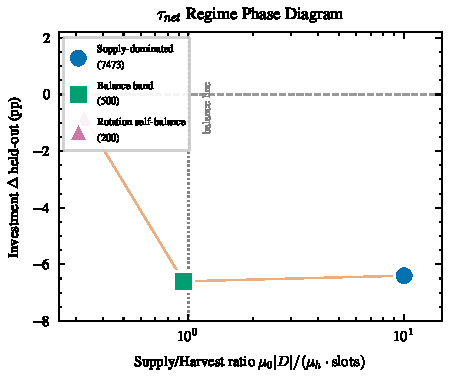
\includegraphics[width=\linewidth]{fig2_phase.pdf}
\caption{$\tau_{net}$ regime phase diagram}
\label{fig:phase}
\end{subfigure}\hfill
\begin{subfigure}{0.49\linewidth}
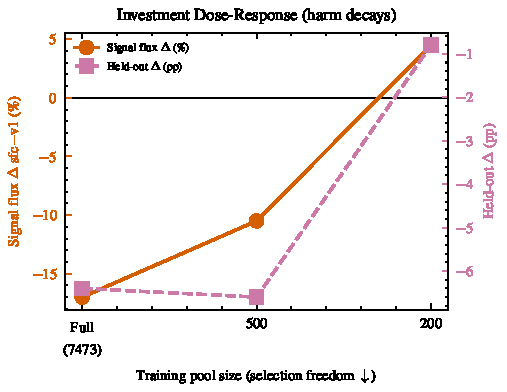
\includegraphics[width=\linewidth]{fig3_dose.pdf}
\caption{Investment dose--response}
\label{fig:dose}
\end{subfigure}
\caption{(a) Three empirical regime points on the supply--harvest plane; investment
harm decreases as the supply/harvest ratio drops. (b) Monotone dose--response:
investment harm decays as selection freedom collapses ($-17\%\to-10.5\%\to+4.5\%$
signal flux; held-out $-6.4\to-6.6\to-0.8$\,pp).}
\label{fig:phasedose}
\end{figure}

\begin{figure}[t]
\centering
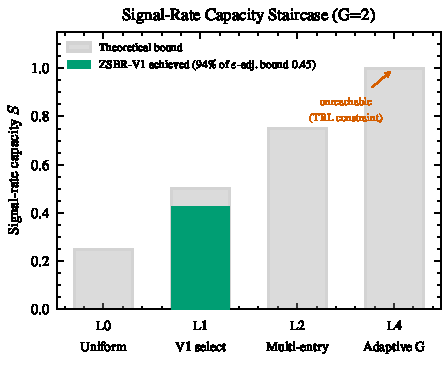
\includegraphics[width=0.62\linewidth]{fig4_capacity.pdf}
\caption{Signal-rate capacity staircase ($G{=}2$). ZSBR-V1 achieves 94\% of the
$\varepsilon$-adjusted L1 selection bound; L4 (per-prompt adaptive $G$) is
unreachable without trainer surgery, and multi-selection (L2/L3) raises coverage
but not the group-level rate (Table~\ref{tab:staircase}).}
\label{fig:capacity}
\end{figure}

\section{Key Findings and Practical Implications}\label{sec:find}

\paragraph{Milestone ledger.} Table~\ref{tab:ledger} consolidates the accuracy
trajectory with its justification at each layer.

\begin{table}[t]
\centering\small
\caption{Milestone ledger (GSM8K test[:500], batch 32; Qwen2.5-3B-Instruct).}
\label{tab:ledger}
\begin{tabular}{@{}lllc@{}}
\toprule
Stage & Configuration & Justification & Held-out \\
\midrule
Base & No training & --- & 23.2\% \\
+Throughput & DGBB gen128, uniform, 100 steps & 97.6\% of wall argmax & 33.3\%$\pm$1.1 \\
+Signal & ZSBR-V1, 100 steps, 3 seeds & 94\% of $G{=}2$ capacity & 40.5\%$\pm$0.9 \\
+Long train & ZSBR-V1, 500 steps & supply-dominated, no depletion & \textbf{45.6\%} \\
\bottomrule
\end{tabular}
\end{table}

\paragraph{When NOT to use curriculum.} Combining \eqref{eq:taunet} and
Theorem~\ref{thm:cap}: if the dataset is trained with cooldown-based greedy
scheduling and $\mu_0|D| \ge \mu_h\cdot\text{slots}$ (or the pool is small enough
for rotation capping to bind), then the signal rate plateaus or rises (no
depletion), any investment incurs opportunity cost without compensation, and pure
greedy is optimal. Both scalars ($\mu_0$ from fzs slope, $\mu_h$ from
re-encounter conversion frequency) are free byproducts of logged training. This is
the first applicability criterion of its kind; prior selection methods
implicitly assume the opposite regime.

\paragraph{Data efficiency.} Pool-500 ZSBR-V1 reaches 45.4\% versus the full
7473-pool's 45.6\%---6.7\% of the data for the same outcome ($15\times$ data
efficiency), with the lossless lower bound located in $(200,500]$ by the pool-200
run (37.4\%, $-8$\,pp, no pathological signature, reward still rising: attributed
to knowledge coverage rather than depletion harm, confound declared
pre-registration).

\paragraph{Negative results as positive evidence.} The first round's 13
pre-registered predictions (F: 6, G: 3, H: 4) yielded 12 failures or
undecidables---yet every failure converges on one picture: \emph{supply dominates,
investment is unnecessary, greedy suffices}. A theory that predicts its own
algorithm's failure (SFC, predicted no-gain after calibration, measured
$-6.4$\,pp) and the structural unreachability of its own motivating phenomenon
(depletion) is exhibiting predictive content, not curve-fitting.

\section{Methodology: Pre-registration and Audit Protocol}\label{sec:method}
Six principles, refined across three audit rounds: (1) mandatory prior-art search
plus written novelty declaration before any theoretical commitment; (2)
timestamped pre-registered falsifiable predictions with numeric thresholds, saved
before running; (3) honest clauses---``undecidable'' is a legitimate verdict when
a calibrated window cannot observe the predicted effect (exercised for F-a);
(4) same-round, same-card, same-metric comparisons (ROCm same-seed re-runs diverge
by ${\approx}3$\,pp due to non-deterministic backward atomics, so all contrasts are
paired within a round); (5) post-experiment full raw-data recomputation plus
three-perspective code review; (6) measurement before correction (the rollout
correlation hypothesis was directly measured and falsified before the attribution
was revised).

\paragraph{Metrics.} All fzs figures use the pre-registered segment-fit metric:
first $2/3$ vs.\ last $1/3$ of the trajectory; rebound $=$ late-segment mean minus
trajectory minimum (in pp). Recomputation from raw \texttt{reward\_log} files
matches reported values within $\pm0.4$\,pp. Evaluations save per-item correctness
vectors, enabling McNemar paired tests from the pool-500 round onward
($\chi^2{=}12.64$, $p{<}0.001$ for the SFC harm; $\chi^2{=}0.18$, n.s., at pool
200).

\paragraph{Audit trajectory.} Round E-F: 1 overturned verdict + 5 biases found and
fixed (metric substitution, selective reporting, semantic drift of stratification
keys). Round E-G: 2 Critical + 3 Warning fixed (``untrained'' semantics
contamination of the relay measurement; arm-selective reporting replaced by
all-arm disclosure with bootstrap CIs). Round E-H: \textbf{zero defects}---the
first clean audit, attributed to pre-experiment three-perspective review catching
a naming trap before execution. The trajectory is itself evidence that the
protocol self-corrects.

\paragraph{Novelty re-audit.} A post-experiment re-search found GRESO's priority
on pre-rollout zero-variance filtering, which the writing draft had missed; the
positioning was corrected (independent rediscovery; incremental claims restricted
to the scorer ablation, capacity theory, and regime criterion), and the lesson was
institutionalized as principle (1).

\section{Threats to Validity}\label{sec:threats}
\paragraph{Task and hardware scope.} All training uses GSM8K with rule-based
numeric rewards on one GPU model; the capacity staircase constants and $\mu_0$
interval are dataset-specific. Cross-architecture transfer (\S\ref{sec:l1-adopt},
\S\ref{sec:l3-c3}) tests form portability, not cross-task generality; MATH/code
tasks with different pass-rate distributions may shift $S_0$ and the regime
boundaries.
\paragraph{Seed and environment confounds.} The 500-step milestone is single-seed;
three-seed 500-step runs span 40.4--45.6\% (mean 43.3\%, $\sigma{=}2.6$\,pp), and
seeds 7/123 ran under a rebuilt software environment, so part of that variance may
be environment-induced. All pairwise effects used for verdicts exceed $2\sigma$ of
the relevant round, per the pre-registered single-seed clause.
\paragraph{Non-determinism.} Same-seed same-config re-runs diverge by
${\approx}3$\,pp on ROCm (backward atomics); all reported contrasts are therefore
same-round paired, and re-run checks are labeled as such in the scorecard.
\paragraph{Metric limitations.} fzs counts investment slots as zero-signal by
construction (mechanic, not dynamics---flagged for F-f); the binary pass-rate
approximation under-estimates signal from format-split groups; the $\tau_{net}$
derivation treats compositions as quasi-static within a cycle.
\paragraph{Single-seed regime points.} Pool-200/500 regime verdicts rest on one
seed each, with effect sizes $\gg2\times$ the measured 100-step seed noise; the
pre-registered clause accepts this for sign determination only.
\paragraph{Independent rediscovery.} ZSBR's skeleton overlaps GRESO; we claim the
increments listed in \S\ref{sec:bg-related}, not the direction itself.

\section{Limitations and Future Work}\label{sec:limits}
The capacity staircase and capping theorem are validated at $G{=}2$; a closed-form
$G{=}4$ posterior-expectation scorer is derived ($L_1(G{=}4){=}0.875$,
$S_0(G{=}4){=}0.212$ measured) but not trained end-to-end. The depletion regime
itself remains unobserved under any schedule (Corollary~\ref{cor:unreach} says it
cannot be, with cooldown); whether cooldown-free long-horizon training on tiny
pools exhibits it, and whether investment turns positive there, is open. The
chart-generation application direction was re-scoped as future work after a
pre-registered gate rejected the visual-transcription task as ill-posed. Since
autoregressive generation dominates step time, lossless speculative decoding
inside the rollout is a natural fourth layer; a first measurement of drafter
acceptance $\alpha(t)$ across training checkpoints shows
\emph{distribution-specific reallocation} rather than monotone decay
(task-distribution acceptance rises as the policy learns reusable templates;
held-out acceptance falls), suggesting speculative-rollout gains must be modeled as
regime-dependent, mirroring the $\tau_{net}$ structure.

\section{Conclusion}\label{sec:concl}
Effective RLVR is achievable on a single consumer GPU through systematic
layer-by-layer optimization. The key insight is the \emph{progressive-limit
methodology} itself: by exhausting each layer's ceiling before descending, we
arrive at the counterintuitive conclusion that the simplest scheduler (greedy with
cooldown) is optimal under realistic constraints---a conclusion that required a
capacity theory, a dynamics model, and an impossibility theorem to establish
rigorously. For practitioners: use posterior-expectation greedy selection with
${\approx}500$ well-chosen prompts, and do not invest in curriculum---in the
supply-dominated regime it is pure opportunity cost.

\bibliographystyle{plainnat}
\bibliography{refs}

\appendix

\section{Complete Prediction Scorecard}\label{app:scorecard}
All thresholds were timestamped before execution. Verdict symbols: \checkmark\
confirmed, $\times$ falsified, U undecidable under the honest clause.
\begin{center}\small
\begin{tabular}{@{}llll@{}}
\toprule
\# & Prediction & Measured & Verdict \\
\midrule
F-a & fzs rebound $\ge$+3pp & $-3.4$pp & U ($\tau{\approx}2500{\gg}500$; supply branch found) \\
F-b & plateau RMSE$<$5pp & 5.2pp & $\times$ (marginal; $\mu_0$ 4$\times$ underestimated) \\
F-c & sfc signal $\ge$v1+5\% & $-17\%$ & $\times$ \\
F-d & sfc held-out $\ge$v1$-$1pp & $-6.4$pp & $\times$ (net harm, $z{=}2.05$) \\
F-e & conversion calib.\ $R^2\ge$0.7 & $R^2<0$ (1.54$\times$ overest.) & $\times$ (audit re-judged) \\
F-f & sfc$\approx$v1 first 100 & 5.2pp & $\times$ (metric caveat) \\
G-a & pool500 fzs rebound $\ge$+3pp & $-4.1$pp & $\times$ (balance branch) \\
G-b & sfc500 flux $\ge$+5\% & $-10.5\%$ & $\times$ (McNemar $p{<}0.001$) \\
G-c & $n_{eff}$ calib.\ err.\ $<$10pp & 17.1pp & $\times$ (selection bias; $n$-dependent) \\
H-a & pool200 fzs rebound $\ge$+3pp & $-0.5$pp & $\times$ (rotation balance) \\
H-b & sfc200 flux $\ge$+5\% & $+4.5\%$ & $\times$ (marginal; inertia) \\
H-c & v1(200) held-out $\ge$40\% & 37.4\% & $\times$ (bound $\in(200,500]$) \\
H-d & plateau $\mu_0\in[0.002,0.008]$ & 0.0081 & $\times$ (0.0001 over; in CI) \\
A1-a & nocool rebound $\ge$+3pp & $+4.09$pp & \checkmark\ (net $-0.92$\,pp vs.\ cooldown) \\
A1-b & held-out equivalence band & $+0.6$pp & \checkmark\ (equivalence) \\
A1-c & p200 plateau broken $\ge$3pp & $-15$pp & \checkmark\ (+3.8\,pp held-out, 1 seed) \\
A3 & 3-seed mean $\in[43.5,47.5]\%$ & $43.3\%{\pm}2.6$ & $\times$ (marginal; env confound) \\
A4 & data lower bound $\in(300,400]$ & directional & directional obs.\ (cross-round) \\
C1 & DGBB form transfer $R^2\ge0.95$ & $0.9983$ & \checkmark\ (form portable) \\
C2 & ZSBR held-out gain $>0$ (E2B) & $-0.40$pp & $\times$ ($S_0$-compression; $4\times$ var.\ down) \\
C3-a & pool7473 plateau $<10$pp & $-2.8$pp & \checkmark\ (supply plateau) \\
C3-b & pool500 depletion $\ge10$pp & $-2.1$pp & $\times$ (boundary $<500$) \\
\bottomrule
\end{tabular}
\end{center}
First round: 1 undecidable + 12 $\times$, all converging to one self-consistent
picture; every $\times$ produced a documented theoretical refinement. WS-A
follow-up: 3/5 confirm (capping holds in the balanced regime; its pool-size
boundary characterized at 200), one marginal under environment confound, one
directional. WS-C: 2/4 confirm portability; the two $\times$ locate the
model-specific parameters to re-measure.

\section{Run Inventory}\label{app:runs}
All runs: RX 7900 XTX, gen128 (pdb4, ga32), $G{=}2$, LoRA on
Qwen2.5-3B-Instruct unless noted; evaluation GSM8K test[:500], batch 32.
Artifacts (\texttt{config.json}, \texttt{timing.json},
\texttt{efficiency\_report.json}, \texttt{reward\_log.jsonl}, per-item
correctness vectors) are released in the repository under
\texttt{results/}.
\begin{center}\small
\begin{tabular}{@{}llll@{}}
\toprule
Run & Steps & Pool & Key numbers \\
\midrule
uniform s42/s7/s123 & 100 & 7473 & held-out 31.0/33.2/34.0\% \\
zsbr\_v1 s42/s7/s123 & 100 & 7473 & held-out 39.6/41.4/40.6\% \\
zsbr\_v1.0 point-est & 100 & 7473 & fzs 0.708 (ablation failure) \\
zsbr\_v2 s42 & 100 & 7473 & held-out 40.2\%, dup slots 0 \\
zsbr\_v1\_500 s42 & 500 & 7473 & held-out 45.6\% (228/500) \\
zsbr\_sfc\_500 s42 & 500 & 7473 & held-out 39.2\%, $-6.4$\,pp \\
zsbr\_v1\_500\_p500 s42 & 500 & 500 & held-out 45.4\% ($15\times$ eff.) \\
zsbr\_sfc\_500\_p500 s42 & 500 & 500 & held-out 38.8\%, $-6.6$\,pp \\
zsbr\_v1\_500\_p200 s42 & 500 & 200 & held-out 37.4\% \\
zsbr\_sfc\_500\_p200 s42 & 500 & 200 & held-out 36.6\%, n.s. \\
p200 cool/nocool pair & 500 & 200 & plateau $-15$\,pp; held-out $+3.8$\,pp \\
E2B uniform/zsbr & 100 & 7473 & 29.27/28.87\%, $\sigma$ $1.2{\to}0.3$\,pp \\
E2B zsbr p7473/p500 & 500 & --- & fzs plateaus $-2.8$/$-2.1$\,pp \\
DGBB 2D sweep (9 pts) & 10 & 7473 & fit residuals $\le$3.3\%; probe (8,256) \\
\bottomrule
\end{tabular}
\end{center}

\end{document}
